Optimization, as defined by Papadimitriou and
Steiglitz~\cite{papadimitriou1998combinatorial}, is the task concerning the
search for the optimal configuration or set of parameters that maximizes or
minimizes a given objective function. In other words, optimizing involves
finding the~\textquote{best} solution to a given problem among a set of feasible
solutions. Formally, an optimization problem can be defined as follows:

\begin{definition}[Optimization Problem~\cite{papadimitriou1998combinatorial}]
  \label{def:optimization-problem}
  An optimization problem is a tuple $(\mathcal{S}, f)$, where
  $\mathcal{S}$ is a set containing all feasible solutions, and $f$ is an
  objective (cost) function, with a mapping such that:

  \begin{equation}
    \label{eq:optimization-problem}
    f \colon \mathcal{S} \longrightarrow \mathbb{R}
  \end{equation}

  That is, each solution $s \in \mathcal{S}$, is assigned a real value
  representing its quality, with the highest quality solution $s^{*} \in
    \mathcal{S}$ being referred to as the global optimal solution or just global optimum.
\end{definition}

\begin{definition}[Global Optimum~\cite{hiriart-urruty1995conditions,papadimitriou1998combinatorial}]
  \label{def:global-optimum}
  Assuming, without loss of generality, an optimization problem with a maximizing
  objective function a global optimum $s^* \in \mathcal{S}$ is expressed by:

  \begin{equation}
    \forall s \in \mathcal{S} \colon f(s^{*}) \geq f(s)
  \end{equation}

\end{definition}

Since Google Hash Code problems~\cite{googlellc2023codingcompetitionsarchive}
have a single-objective maximizing objective function, we will only consider
maximization in this work. However, it is possible to reformulate problems with
a minimizing objective function for maximization~\cite{nocedal2006numerical}
using the identity:

\begin{equation}
  \label{eq:max2min}
  \max{-f(s)} = \min{f(s)}
\end{equation}

\subsection{Combinatorial Optimization}
\label{sec:combinatorial-optimization}

Optimization problems can be divided into~\textit{discrete}
and~\textit{continuous} based on the domain of their variables. In problems with
~\textit{discrete} variables, solutions are defined on a finite, possibly
countably infinite, set of values~\cite{papadimitriou1998combinatorial}. As for
problems with~\textit{continuous} variables, the solutions take on any value on
a continuous (infinite) subset of real numbers. Nevertheless, there are problems
that involve both~\textit{discrete} and~\textit{continuous} variables, commonly
denominated as mixed~\cite{nocedal2006numerical}.

\acrfull{combinatorial-optimization} problems are a subset of optimization
problems characterized by a discrete solution space that typically involves
different permutations, groupings, or orderings of objects that satisfy some
problem-specific criteria~\cite{papadimitriou1998combinatorial,vieira2009uma}.
As such, solutions for these problems are represented objects related to the
combinatorics~\eg{} integers, permutations sets and
graphs~\cite{blummetaheuristics,yu2010combinatorial}. Thus, regarding the
previous definition of an optimization problem,
a~\acrshort{combinatorial-optimization} can be formally defined as follows:

\begin{definition}[Combinatorial Optimization Problem~\cite{papadimitriou1998combinatorial}]
  \label{def:combinatorial-optimization-problem}
  A combinatorial optimization problem is an optimization
  problem~(\ref{def:optimization-problem}) where the set $\mathcal{S}$ of
  feasible solutions is finite or countably infinite.
\end{definition}

Typical examples of~\acrshort{combinatorial-optimization} problems include
network flow, matching, scheduling, shortest path and decision problems.
Notably, the~\acrfull{knapsack-problem} is a
well-known~\cite{cacchiani2022knapsack, yu2010combinatorial,festa2014brief}
example of a~\acrshort{combinatorial-optimization} problem where the goal is to
find the subset of items with the highest total profit that can fit in a
knapsack without exceeding its maximum capacity.

Due to the inherent discreteness of decision spaces
within~\acrshort{combinatorial-optimization} optimization problems, solutions
can be understood as compositions of objects (components) selected from a finite
set that including all elements capable of contributing to a solution.  This
set, commonly known as the~\textquote{ground set}, can be defined as shown:

\begin{definition}[Ground Set~\cite{outeiro2021application,festa2014brief,marti2013multistart}]
  \label{def:ground-set}
  The ground set $\mathcal{G}$ of a~\acrshort{combinatorial-optimization}
  problem is a finite set of containing all possible components for the problem.

  \begin{equation}
    \label{eq:ground-set}
    \mathcal{G} \colon \{c_{1}, c_{2}, c_{3}, \ldots, c_{i}\}
  \end{equation}
\end{definition}

Hence, within the context of~\acrshort{combinatorial-optimization} problems, a
feasible solution constitutes a subset of the ground set, denoted as $s \in
  \mathcal{S} \subseteq 2^{\mathcal{G}}$, where the included components satisfy
problem-specific constraints. Moreover, a partial solution is defined by its
former capacity to incorporate additional components from the ground set. In
contrast, a complete solution is incapable of accepting further components
without violating feasibility, as opposed to the former which can be infeasible.

To illustrate these concepts, let's consider the practical example of the
\acrshort{knapsack-problem}. In this context, the ground set is the set of all
the available items (components). As such, a feasible solution is one in which
items placed within the knapsack do not exceed its capacity limit. A partial
solution is one where the knapsack is not yet full and additional items can
still be accommodated. Notably, in this case, the partial solution is still
feasible. Finally, a complete solution is a feasible solution where no further
items can be added due to capacity constraints.

In essence, since \acrshort{combinatorial-optimization} problems involve
choosing a combination of objects any algorithm that is able to enumerate the
entirety of the solution space can be used to solve these problems. However,
finding an optimal solution can be difficult, and exhaustive search strategies
may not be able to solve many of these problems, which are often
NP-Hard~\cite{yu2010combinatorial,festa2014brief} and thus not approachable by
algorithms in a reasonable amount of time. In these cases, approximation,
heuristic and~\acrshort{meta-heuristic} methods present themselves as effective
alternatives to be considered.

\subsection{Global and Local Optimization}

With regard to the search of solutions for optimization problems, there are two
primary strategies: \acrfull{global-optimization} and \acrfull{local-optimization}.

\acrshort{global-optimization} involves the process of discovering the ultimate
global optimum~(\ref{def:global-optimum}) for a given problem, regardless of
where it might lie within the solution space. This search for the best solution
is often called~\textit{exploration}. In contrast,
\acrshort{local-optimization} concentrates on finding the most optimal solution
among proximate that are close in some way, which is commonly referred to as
\textit{exploitation}. The concept of proximity is related to the definition
of a neighborhood, which for a given solution is specified by a particular
neighborhood structure defined as follows:

\begin{definition}[Neighborhood Structure~\cite{papadimitriou1998combinatorial, blummetaheuristics}]
  \label{def:neighborhood-structure}

  A neighborhood structure for an optimization problem is a mapping:

  \begin{equation}
    \label{eq:neighborhood-structure}
    \mathcal{N} \colon \mathcal{S} \longrightarrow 2^{\mathcal{S}}
  \end{equation}

  Such that, a set of neighboring solutions $\mathcal{N}(\hat{s}) \subseteq
    \mathcal{S}$ is assigned for each solution $\hat{s} \in \mathcal{S}$. This
  referred to as the neighborhood of $\hat{s}$.
\end{definition}

In general, the neighborhood structure refers to the set of rules that must be
applied to a solution in order to generate all of its neighbors.  Additionally,
we can define a local optimal solution or just local optimum as follows:

\begin{definition}[Local Optimum~\cite{hiriart-urruty1995conditions,blummetaheuristics,nocedal2006numerical}]
  \label{def:local-optimum}

  Assuming maximization without loss of generality, a solution $\hat{s}$ is
  a local optimum with respect to a given neighborhood structure $\mathcal{N}(\hat{s})$ iff:

  \begin{equation}
    \label{eq:local-optimum}
    \forall s \in \mathcal{N}(\hat{s}) \colon f(\hat{s}) \geq f(s)
  \end{equation}

  Furthermore, $\hat{s}$ is a considered a strict a local optimum iff:

  \begin{equation}
    \label{eq:strict-local-optimum}
    \forall s \in \mathcal{N}(\hat{s}) \setminus \{\hat{s}\} \colon f(\hat{s}) > f(s)
  \end{equation}
\end{definition}

As an illustrative example, consider the objective function $f(s)$ shown in~\ref{fig:optima}.
With respect to the~\Cref{def:global-optimum,def:local-optimum}, the solution
$s^1$ is a global optimum and $s^2$, $s^3$ are (strict) local optima.

\begin{figure}[h]
  \centering
  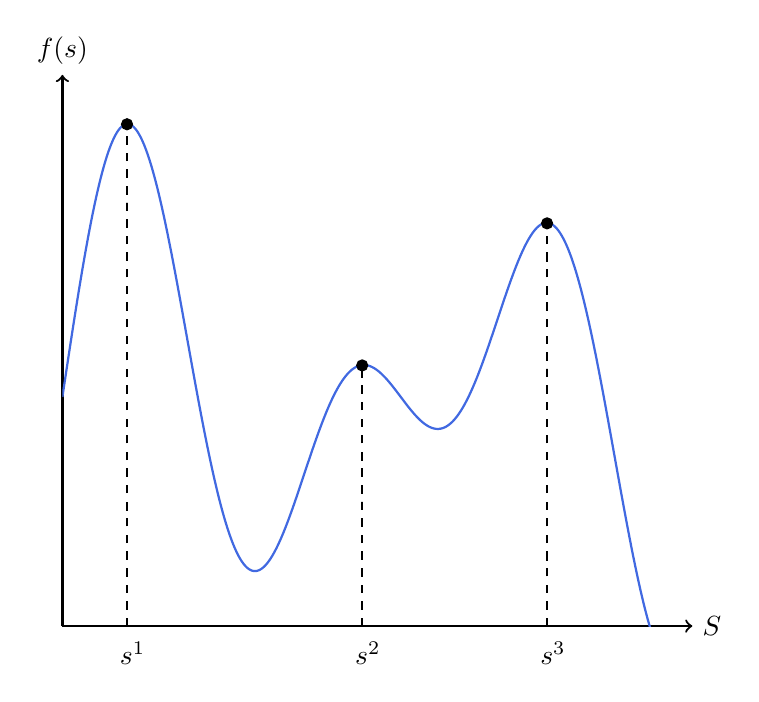
\begin{tikzpicture}
	% Axis Lines
	\draw[->, thick] (0,0) -- (8,0) node[right] {$S$};
	\draw[->, thick] (0,0) -- (0,7) node[above] {$f(s)$};

	\begin{axis}[axis lines = none,scale only axis=true,xmin=0,
			xmax=18.5,ymin=0,ymax=10]

		% Main Plot
		\addplot[domain=0:17,samples=1000,smooth,color=RoyalBlue,
			thick] {2.5*sin(deg(x)) + 2.5*sin(deg((2/3)*x)) + 4};

		% Vertical Line (s1)
		\addplot[domain=0:17,thick,samples=1000,dashed,
			smooth] coordinates {(1.8,0) (1.8,8.76)};
		\addplot[domain=0:17,mark=*] coordinates {(1.8,8.76)};
		% \draw (1.8,8.76) circle[radius=1.5pt];
		% \fill (1.8,8.76) circle[radius=1.5pt];

		% Vertical Line (s2)
		\addplot[domain=0:17,thick,samples=1000,dashed,
			smooth] coordinates {(8.35,0) (8.35,4.55)};
		% \draw (8.35,4.55) circle[radius=1.5pt];
		% \fill (8.35,4.55) circle[radius=1.5pt];
		\addplot[domain=0:17,mark=*] coordinates {(8.35,4.55)};

		% Vertical Line (s3)
		\addplot[domain=0:17,thick,samples=1000,dashed,
			smooth] coordinates {(13.5,0) (13.5,7.03)};
		% \draw (13.5,7.03) circle[radius=1.5pt];
		% \fill (13.5,7.03) circle[radius=1.5pt];
		\addplot[domain=0:17,mark=*] coordinates {(13.5,7.03)};
	\end{axis}

	% Labels
	\node (s1) at (0.89,-0.35) {$s^1$};
	\node (s1) at (3.88,-0.35) {$s^2$};
	\node (s1) at (6.23,-0.35) {$s^3$};

\end{tikzpicture}


  \caption{Global and Local Optima}
  \label{fig:optima}
\end{figure}

In practice, the decision to use either a global or local optimization strategy
is often influenced by factors such as the available time budget and the
preferences of the decision maker. While~\acrshort{global-optimization} aims to
find the optimal solution to a problem, the search process may be time-consuming
or, in some cases, computationally infeasible due to the size of the search
space.  On the other hand,~\acrshort{local-optimization}, while lacking the
optimality guarantees of, is able to quickly generate good solutions that may be
acceptable to the decision maker. Nonetheless, the quality of the solutions may
be poor due to the ruggedness of the objective function fitness landscape (many
local optima). Ultimately, the performance of both methods is closely tied to
problem-specific knowledge.

In the Google Hash Code competition, due to the time imposed by the competition
setting, it is often not in the interest of the contestants to use global
optimization methods, as they are unlikely to finish on more complex problem
instances. Instead, a balance between global and local optimization
(\textit{exploration} and \textit{exploitation}) is typically employed. To
elaborate, the strategy typically involves~\textit{exploring} the search space
via~\acrshort{global-optimization} methods to find \textquote{good} starting
solutions, that~\acrshort{local-optimization} methods can
further~\textit{exploit}.

\subsection{Black-Box and Glass-Box Optimization}

In the field of optimization, two settings are commonly recognized:
\acrfull{black-box-optimization} and \acrfull{glass-box-optimization}.

In \acrshort{black-box-optimization} optimization settings there is no
information about the landscape of the function being optimized, constraints
defining the set of feasible solutions~\cite{alarie2021two} or the objective
function is too complex to be approached from an analytical perspective. As
such, algorithms for achieving solutions for these problems do so only by
interacting with the problem through the evaluation of potential candidate
solutions~\cite{doerr2020complexity}. Meta-Heuristics, as will be later detailed
are examples of methods that follow this approach for finding/improving
solutions. By contrast, in \acrshort{glass-box-optimization} optimization, also
known as \textit{white box} optimization, there is a good understanding of the
problem instance being optimized and the objective function
properties~\cite{doerr2020complexity}. Hence, the algorithms used may take
advantage of more analytical properties of the problem since they are
transparent to the solver.

For the purpose of clarification, with regard to the previously mentioned
\acrshort{knapsack-problem}, a~\acrshort{black-box-optimization} strategy would
entail the utilization of a search heuristic such as simulated
annealing~\cite{luke2013essentialsa} to obtain solutions. This is because the
algorithm only necessitates knowledge of how to evaluate the quality of
solutions through the objective function and not any specific information about
the function being optimized. Alternatively, if the problem were to be
formulated as an~\acrfull{ilp}~\cite{nocedal2006numerical,papadimitriou1998combinatorial}
problem, it would become amenable to a~\acrshort{glass-box-optimization}
approach, as the objective function would be accessible, and additional
information about the problem could be inferred from it and provided to the
algorithm.

In the context of the Hash Code competition, contestants typically engage the
problems from a~\acrshort{black-box-optimization} perspective, as the underlying
objective function of the is too complex to formalize. Additionally, the process
of formalization can be time-consuming and, as a result, the usage of a
~\acrshort{glass-box-optimization} methods post-formalization would not be
justified, as they could turn out to be computationally slower. However, it is
in many cases, possible to use~\acrshort{glass-box-optimization}
methods,~\eg{},~\acrshort{ilp} to tackle sub-problems that are more simple to
formalize as more knowledgeable contestants have demonstrated in the past.
